\subsectionaddtolist{۱.۲ سلسله مراتب کلید در یک سامانه بانکی}

\subsubsection*{آ}
ساختار درختی این سامانه به این صورت است که کلید ریشه از همه محافظت می‌کند:
\begin{itemize}
    \item {سطح ریشه (Root) :} کلید اصلی $MK$ که در داخل ماژول امنیتی سخت‌افزاری شعبه مرکزی تولید و محافظت می‌شود و هرگز به صورت متن آشکار از آن خارج نمی‌شود.
    \item {سطح میانی (Branches) :} کلیدهای $KEK_1, KEK_2, \dots, KEK_n$ برای شعب مختلف. هر $KEK_i$ توسط $MK$ رمز شده و به صورت ایمن در اختیار شعبه مربوطه قرار می‌گیرد (یعنی ذخیره $E(MK, KEK_i)$).
    \item {سطح برگ‌ها (Sessions) :} کلیدهای نشست $DEK_1, DEK_2, \dots$. داده‌های واقعی بانکی با کلید $DEK$ رمز می‌شوند و خود کلید $DEK$ پس از تولید، توسط $KEK$ همان شعبه رمز می‌شود (یعنی $E(KEK, DEK)$).
\end{itemize}

\begin{center}
    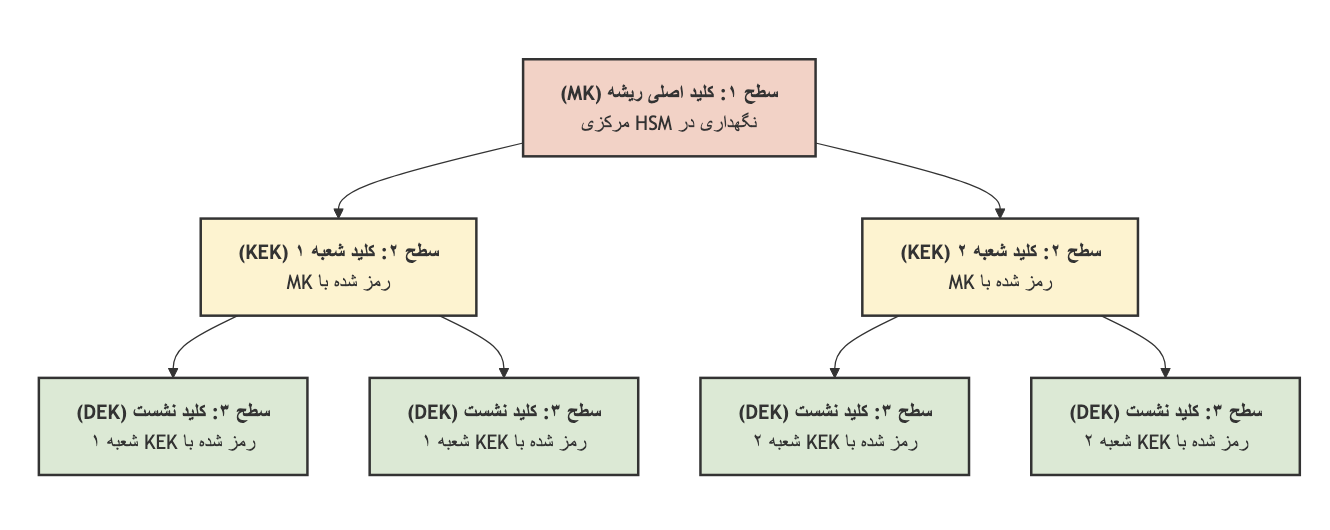
\includegraphics[width=0.8\textwidth]{figs/image.png}
\end{center}

\subsubsection*{ب}
از آنجا که این کلید فقط برای یک نشست خاص است، شعاع تخریب {بسیار محدود} است. تنها داده‌هایی که در همان نشست خاص رد و بدل یا رمز شده‌اند در معرض خطر قرار می‌گیرند. سایر نشست‌های همان شعبه و سایر کاربران کاملا امن می‌مانند.

\subsubsection*{ج}
شعاع تخریب {متوسط تا بزرگ} است. اگر KEK یک شعبه لو برود، مهاجم می‌تواند تمام DEK های آن شعبه را رمزگشایی کند. در نتیجه، تمام تراکنش‌ها و نشست‌های مربوط به آن شعبه خاص به مخاطره می‌افتد. با این حال، اطلاعات سایر شعب بانکی و کلید مستر (MK) همچنان امن هستند.

\subsubsection*{د}
\begin{itemize}
    \item {سطح DEK :} با فرکانس بالا (معمولا به ازای هر تراکنش یا اتصال جدید) یک کلید تصادفی جدید تولید شده و با پایان نشست منقضی می‌شود.
    \item {سطح KEK :} به صورت دوره‌ای (مثلا روزانه یا هفتگی). مرکز، یک KEK جدید تولید کرده، آن را با MK رمز می‌کند و برای شعبه می‌فرستد تا از این به بعد نشست‌های جدید با کلید جدید محافظت شوند.
    \item {سطح MK :} به ندرت (مثلا سالی یک‌بار، یا هنگام احساس خطر و ارتقای سخت‌افزار). تعویض این کلید معمولا نیازمند تشریفات امنیتی موسوم به مراسم کلید (\lr{Key Ceremony}) با حضور همزمان چند نفر از مدیران امنیتی در کنار دستگاه HSM است.
\end{itemize}


\subsectionaddtolist{۲.۲ راهبردهای ذخیره‌سازی کلید}

\subsubsection*{آ}
\begin{itemize}
    \item  محرمانگی {بسیار پایین} (هرکس به دیسک دسترسی یابد کلید را می‌دزدد)، در دسترس بودن {بسیار بالا} (دسترسی سریع و بدون دردسر)، هزینه {بسیار پایین} (هیچ سربار پردازشی یا مالی ندارد).
    \item محرمانگی {متوسط رو به بالا} (وابسته به اینکه KEK کجا نگهداری می‌شود)، در دسترس بودن {بالا}، هزینه {متوسط} (سربار پردازشی برای باز کردن رمز کلید در زمان اجرا).
    \item محرمانگی {بسیار بالا} (کلیدها هرگز از سخت‌افزار استخراج نمی‌شوند)، در دسترس بودن {متوسط/بالا} (وابسته به آپتایم و در دسترس بودن شبکه متصل به سخت‌افزار)، هزینه {بسیار بالا} (خرید، نگهداری و پیچیدگی‌های مدیریت دستگاه‌های گران‌قیمت).
\end{itemize}

\subsubsection*{ب}
\begin{itemize}
    \item  این روش فقط در محیط‌های کاملا ایزوله که هیچ اتصال شبکه‌ای به بیرون ندارند و تهدید سرقت فیزیکی دیسک یا دسترسی از راه دور وجود ندارد قابل استفاده است (مانند سرورهای ایزوله که کل سیستم‌عاملشان از  \lr{Full Disk Encryption} بهره می‌برد و کلید دیسک در بوت‌لودر تامین می‌شود).
    \item برای مقابله با تهدیداتی نظیر سرقت آفلاین دیسک‌ها، لو رفتن دیتابیس یا بک‌آپ‌ها مناسب است. در معماری‌های رایج وب (مانند الگوی \lr{Envelope Encryption}) کاربرد دارد، مشروط بر اینکه KEK در یک متغیر محیطی امن یا یک \lr{Secret Manager} مجزا نگهداری شود.
    \item برای مدل‌های تهدید پیشرفته و مهاجمانی که ممکن است بالاترین سطح دسترسی سیستم را به دست آورند کاربرد دارد. در CA های صدور گواهی و هسته مرکزی سامانه‌های بانکی که قانونا نیاز به تضمین عدم نشت کلید دارند، کاملا الزامی است.
\end{itemize}


\subsectionaddtolist{۳.۲ مشتق‌سازی کلید از راز مشترک}

\subsubsection*{آ}

استفاده مستقیم از راز مشترک $Z$ خروجی دیفی-هلمن به عنوان کلید رمزنگاری به سه دلیل مجاز نیست:
\begin{enumerate}
    \item خروجی تبادل کلید دیفی-هلمن ($Z$) لزوما از نظر توزیع آماری بیت‌ها یکنواخت نیست و ساختار جبری و ریاضی خاصی دارد. در حالی که کلید آماده برای الگوریتمی مثل AES باید کاملا تصادفی و غیرقابل پیش‌بینی باشد.
    \item  ما برای برقراری یک کانال امن به سه مقدار مجزا (کلید رمزنگاری AES ، کلید احراز اصالت MAC و بردار مقداردهی اولیه IV ) نیاز داریم. بر اساس اصول رمزنگاری، نباید از یک مقدار واحد ($Z$) برای چندین هدف مختلف استفاده کرد؛ چرا که تعامل این پروتکل‌ها با یک کلید واحد می‌تواند منجر به نشت اطلاعات یا حملات متقاطع شود.
    \item  کلیدهای نهایی باید به متن و بافتار نشست (مانند نانس‌های تبادل شده و هویت دو طرف) وابسته باشند. اگر از $Z$ به تنهایی استفاده شود، کلید بین نشست‌های مختلف یا موازی کاملا مستقل و قاطی نخواهد شد و این موضوع ریسک حملاتی مثل Replay یا تشابه کلید در نشست‌های موازی را بالا می‌برد.
\end{enumerate}


\subsubsection*{ب}

بهترین و استانداردترین روش، استفاده از یک تابع مشتق‌ساز کلید بر پایه هَش استاندارد است. فرآیند تولید کلیدها به این صورت انجام می‌شود:

\begin{enumerate}
    \item {مرحله استخراج (Extract) :} ابتدا آنتروپی راز مشترک $Z$ به کمک یک نمک ($salt$) استخراج می‌شود تا یک کلید شبه‌تصادفی اولیه ($PRK$) تولید شود:
    $$PRK = HKDF-Extract(salt, Z)$$
    که در آن برای گره زدن کلید به بافتار نشست فعلی، مقدار $salt$ را از هَش کردن نانس‌های طرفین و کل تاریخچه پیام‌های رد و بدل شده ($transcript$) به دست می‌آوریم:
    $$salt = H(N_A \parallel N_B \parallel transcript)$$
    
    \item {مرحله بسط (Expand) :} در این مرحله از روی $PRK$، برای هر یک از اهداف مورد نیاز خروجی‌های مجزایی با طول مشخص و با استفاده از برچسب‌های متنی متفاوت و اطلاعات کانتکست استخراج می‌کنیم تا کلیدها از نظر رمزنگاری کاملاً مستقل باشند:
    $$K_{enc} = {HKDF-Expand}(PRK, {'AES key'} \parallel context, 32)$$
    $$K_{mac} = {HKDF-Expand}(PRK, {'HMAC key'} \parallel context, 32)$$
    $$IV_0 = {HKDF-Expand}(PRK, {'IV'} \parallel context, 16)$$
\end{enumerate}

به این ترتیب، کلید رمزنگاری ($K_{enc}$)، کلید احراز اصالت ($K_{mac}$) و بردار مقداردهی اولیه ($IV_0$) کاملاً تفکیک شده و مستقل از یکدیگر خواهند بود. 

برای پیام‌های مختلف در طول نشست نباید از یک $IV$ تکراری استفاده شود؛ بنابراین یا باید برای هر پیام یک $IV$ اختصاصی و جداگانه مشتق شود و یا اینکه از یک \lr{Sequence Number} یا شمارنده به صورت \lr{XOR} با $IV_0$ کمک گرفته شود تا از حملات مربوط به تکرار بردار اولیه جلوگیری به عمل آید.

\subsectionaddtolist{۴.۲ فضای کلید مؤثر}

\subsubsection*{آ}
مهاجم بازه زمانی تولید کلید را می‌داند که معادل ۱ ساعت یا $۳۶۰۰$ ثانیه است. دقت تابع زمان نیز ۱ میلی‌ثانیه است. از آنجا که Seed این مولد تنها بر اساس زمان است، تعداد Seed های ممکن به صورت زیر محاسبه می‌شود:
$$  \frac{3600 \text{ s}}{0.001 \text{ s}} = 3,600,000 $$
بنابراین فضای کلید مؤثر برابر $3.6 \times 10^6$ حالت است که به توان ۲، رقمی حدودا برابر با $2^{21.7}$ می‌شود.

\subsubsection*{ب}
فضای کلید واقعی و تئوری برای الگوریتم \lr{AES-128} برابر با $2^{128}$ حالت است. اما استفاده از زمان سیستم به عنوان Seed ، فضای جستجو را از $2^{128}$ به عدد فاجعه‌بار $2^{22}$ کاهش داده است.

این سیستم کاملا شکسته است. یک مهاجم اصلا نیازی به حمله Brute-force روی کل $2^{128}$ حالت ندارد؛ بلکه کافیست ۳ میلیون عدد زمان را به عنوان Seed در اسکریپت خود وارد کرده، کلیدها را تولید و امتحان کند. این کار روی یک سیستم کامپیوتری معمولی در کسری از ثانیه انجام می‌شود. پیامد این اشتباه این است که توسعه‌دهنده به جای استفاده از تولیدکننده‌های امن رمزنگاری مانند ماژول secrets ، از توابع ساده random استفاده کرده.